% Figure from MATH 556 notes, section 20. Compile with the notes preamble.
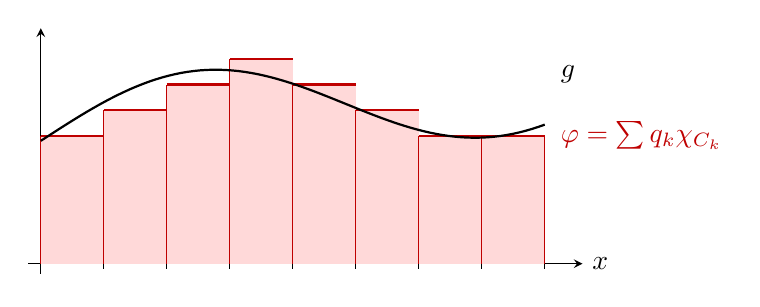
\begin{tikzpicture}[x=1.6cm, y=1.3cm, >=stealth]
    \draw[->] (-0.1,0) -- (4.3,0) node[right] {$x$};
    \draw[->] (0,-0.1) -- (0,2.3);
    \foreach \k in {0,...,7} {
        \pgfmathsetmacro{\xa}{0.5*\k}
        \pgfmathsetmacro{\c}{1.2+0.5*sin(deg(0.5*\k*1.3))+0.15*(0.5*\k)}
        \pgfmathsetmacro{\q}{round(\c*4)/4}
        \fill[red!15] (\xa,0) rectangle (\xa+0.5,\q);
        \draw[red!75!black, thick] (\xa,\q) -- (\xa+0.5,\q);
        \draw[red!75!black] (\xa,0) -- (\xa,\q);
    }
    \draw[red!75!black] (4,0) -- (4,{round((1.2+0.5*sin(deg(3.5*1.3))+0.15*3.5)*4)/4});
    \draw[thick, domain=0:4, samples=80] plot (\x, {1.2+0.5*sin(deg(\x*1.3))+0.15*\x});
    \node[anchor=west] at (4.05,1.85) {$g$};
    \node[red!75!black, anchor=west] at (4.05,1.25) {$\varphi = \sum q_k \chi_{C_k}$};
    \foreach \x in {0,0.5,...,4} \draw (\x,0) -- (\x,-0.05);
\end{tikzpicture}
